%!TEX root = ../thesis.tex
%*******************************************************************************
%****************************** Second Chapter *********************************
%*******************************************************************************

\chapter{The SNO+ Detector}\label{chap:detector}
\section{Detector Geometry and Design}
The SNO+ detector is a large, multi-purpose neutrino detector built in the SNOLAB underground laboratory near Sudbury, Canada. Its main detector structure is taken from the Nobel prize-winning Sudbury Neutrino Observatory (SNO)~\cite{}, % cite nobel prize for Art
and can be seen in Fig.~\ref{fig:snoplus_detector}.

\begin{figure}
    \centering
    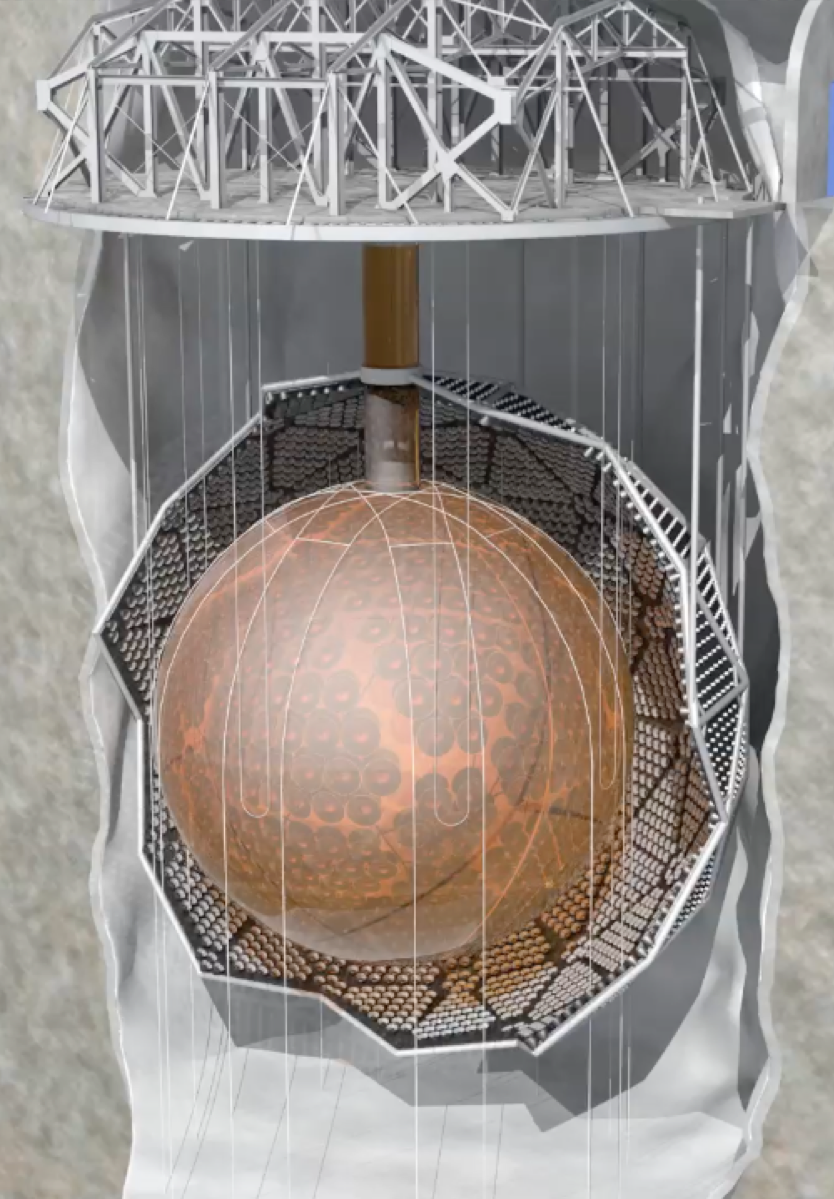
\includegraphics[width=0.48\linewidth]{2_Detector/Figs/detector_picture.png}
    \caption[3D model of the SNO+ detector]{3D model of the SNO+ detector~\cite{albanese_sno_2021}.}
    \label{fig:snoplus_detector}
\end{figure}


\begin{itemize}
    \item Describe the SNO+ geometry at a high level: explain structure, and why certain design choices were made.
    \item Describe standard coordinate axis; note AV offset.
    \item Mention the main phases of SNO+, both past, present, and future.
\end{itemize}
\section{Detecting a Physics Event in SNO+: A Journey}
\begin{itemize}
    \item Begin the ``journey of a SNO+ Physics Event'' --- starting by explaining how a high-energy particle interacts with matter to generate Cherenkov and/or scintillation light. In both cases, optical wavelength light gets generated.
    \item Then, light propagates through the detector, possibly undergoing various physics processes: Rayleigh scattering, absorption, re-emission, refraction, and reflection.
    \item Light gets detected via the PMTs: explain how.
    \item Thus begins the DAQ chain. Signals reach the crates of electronics on deck and are processed. A ``sufficient signal'' leads to the triggering of the detector, which then enables for the saving of the event's information via the event builder.
\end{itemize}
\section{Calibrations and Detector Modelling}
\begin{itemize}
    \item I now describe how calibrations enable us to use the stored data for actual physics.
    \item Detector's state is continuously monitored via a number of systems for data quality purposes, including a human detector `shifter'. Mention use of run numbers. CHS and CSS ensure only ``good'' channels used in any analysis.
    \item First main set of calibrations are the ECAs and PCAs. These help us convert raw electronic signal information from PMTs into `calibrated' hit times and charges. PCAs performed via TELLIE and the Laserball.
    \item These initial calibrations allow for the first two passes of data processing. SMELLIE data comes from this part of the processing chain.
    \item In order to infer properties of an underlying physics event, an accurate model of the detector is needed. This requires two things: a set of calibration tools, and a piece of simulation software. The latter is RAT (explain briefly).
    \item Aims of remaining calibration tools are to obtain the optical parameters necessary for accurate modelling. Go through briefly all the calibration tools we have available: SMELLIE, AMELLIE, the Laserball, the AmBe and N16 sources, and in situ backgrounds.
    \item Using RAT once calibrated, event reconstruction can become possible. Briefly describe how energy, position, and time reconstruction works. Mention existence of direction fitting!
\end{itemize}